Chapter 1 established the theoretical results and stated the remaining gaps.
Chapter 2 tested small cases and searched larger ones for dense examples.
This chapter brings those strands together.
It identifies the main conclusions and separates the central open problems from questions of classification and completeness.

\section{The directed frontier}
The simple directed arc problem has several verified dense constructions, but
their feasibility must not be confused with optimality. A construction proves
a lower bound: it shows that at least that many arcs are possible. Proving the
extremal value would additionally require an upper bound for every feasible
digraph.

\begin{construction}[Competing dense directed families]\label{const:directed-comparison}
For $n\ge m\ge2$, choose the densest of the directed hub, the augmented
bipartite digraph and the clique-core digraph
(\Cref{const:directed-hub,const:augmented-bipartite,const:clique-core}).
Their respective arc counts are
\[
 H_m(n)=m(n-1),\qquad
 Q_m(n)=\floorfrac{(n+m-2)^2}{4},\qquad
 B_m(n)=\floorfrac{(n+m-3)^2}{4}+2(m-1).
\]
Each has maximum local arc-connectivity $m-1$. Consequently,
\[
 \ell_m^{\mathrm{dir}}(n)\ge \max\{H_m(n),Q_m(n),B_m(n)\}.
\]
This is a lower bound, not a proposed formula for the optimum.
\end{construction}

The earlier conjecture asserted $\ell_m^{\mathrm{dir}}(n)=
\max\{H_m(n),Q_m(n)\}$ for every $n\ge m$. It is false.
The clique-core construction, supplied by Stijn Cambie, has $57$ arcs at
$m=5$, $n=12$, with maximum local arc-connectivity $4$. The proposed formula
gives only $56$. More generally, this construction beats both earlier families
whenever $m\ge5$ and $m+7\le n\le3m-3$
(\Cref{const:clique-core}). It does not prove that $57$ is optimal at $(12,5)$,
nor that the maximum of all three displayed counts is always optimal.

For fixed $m$, the augmented bipartite family eventually has more arcs than
the other two displayed families. That comparison only ranks these
constructions. Another feasible family could still be denser.
Cambie also supplied an AI-assisted argument for eventual optimality.
It is retained separately as a research note, not used as a theorem or
adopted as a conjecture in this thesis.
At $m=2$, the exact value is already established by
\Cref{thm:dir-arc-m2-exact}: the bipartite count is optimal for $n\ge7$.
\Cref{fig:crossover} compares the hub and augmented bipartite counts at $m=3$.

\begin{figure}[t]
    \centering
    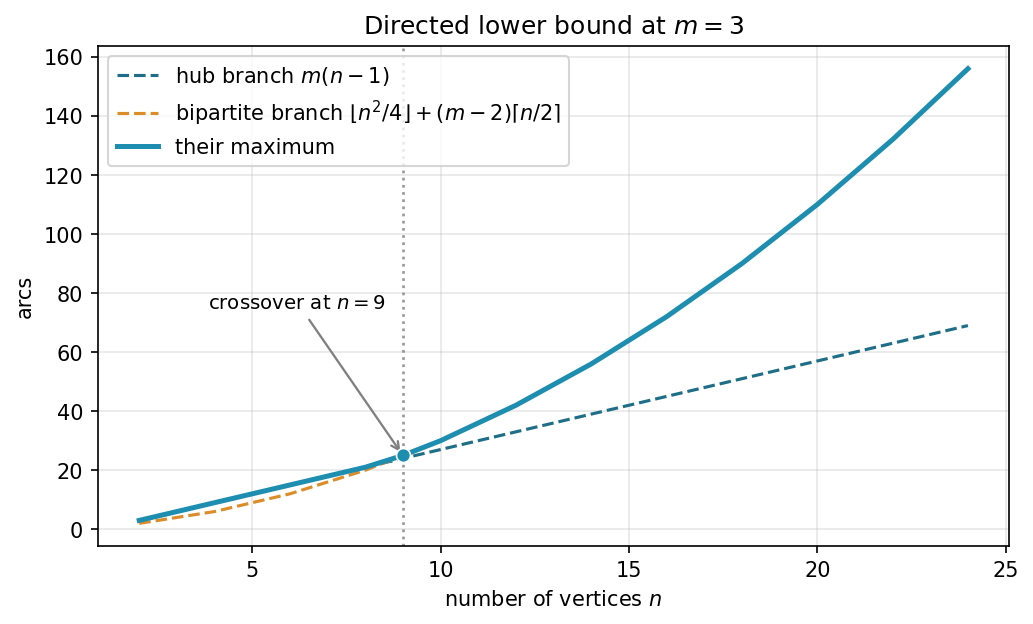
\includegraphics[width=0.78\textwidth]{figures/directed_crossover.png}
    \caption{The hub and augmented bipartite lower bounds at $m = 3$, and their maximum. The plot asserts no upper bound.}
    \label{fig:crossover}
\end{figure}

At $m=3$, exhaustive search proves the values $6,9,12,15$ for $n=3,4,5,6$.
The two separation conditions agree at every one of these orders (\Cref{rem:dir-vertex-m3}).
The search does not settle $n=7$.

The earlier decomposition conjecture has been removed as well.
It would force the quadratic upper bound as soon as that branch exceeds the
hub bound, which already happens at $m=5$, $n=12$.
The counterexample therefore refutes that structural assertion too.

The augmented bipartite count has the same leading term and the same order of error as the optimum.
\Cref{thm:dir-arc-linear-error} proves this without assuming the shape of an extremal graph.
The linear coefficient remains unknown among the results proved in this thesis.
Even identifying it would leave the exact bounded correction to establish.
More precisely, the construction gives a linear contribution $(m-2)n/2+O_m(1)$ above $n^2/4$, while the proved upper bound allows $4(m-1)n$. These inequalities do not show that a unique limiting linear coefficient exists.
Once $n$ is large in terms of $m$, the Tur\'an theorem of Huang and Lyu \cite{HuangLyu26} lowers the upper end to $m-1$ (\Cref{ch:basecases}).
The next section considers the separate question of extremal shape.

The directed vertex problem has the same leading term and error order by \Cref{thm:dir-vertex-linear-error}.
\Cref{app:proofs} treats it separately from the arc problem.
It remains open whether the two values are exactly equal for $m \ge 3$.

Allowing parallel arcs closes the arc-disjoint problem completely.
\Cref{thm:dir-multi-full} gives the exact value for every $n \ge 2$ and $m \ge 2$.

\section{Why direction makes the value quadratic}

In an undirected graph, every edge contributes to the degree of both endpoints.
Mader's theorem turns this symmetry into the linear cap $\floor{m(n-1)/2}$.
A digraph has no corresponding symmetry.

In \Cref{const:bipartite}, all arcs go from one part to the other and none return.
A directed route can therefore cross between the parts only once.
The construction has $\floor{n^2/4}$ arcs at $\lec^{\max}=1$.
No undirected graph of connectivity one can have quadratic size.
The linear cap does not survive the introduction of direction.
At $m=2$ and $n=8$, the one-directional construction has $16$ arcs while the hub has $14$.
The directed value must therefore follow the larger branch.

\Cref{const:augmented-bipartite} extends this idea to every $m$.
Each vertex of the larger part receives $m-2$ extra in-arcs from within that part.
\Cref{fig:augmented-wall} draws the construction.
The added arcs provide $m-2$ short detours for each relevant pair.
They raise $\lec^{\max}$ to $m-1$ and the arc count to $\floor{(n+m-2)^2/4}$.
At $m=3$ and $n=10$, the construction has thirty arcs while the hub has twenty-seven.

\begin{figure}[t]
\centering
\begin{tikzpicture}[>=Stealth, scale=1.0,
    wallarc/.style={gdirfaint},
    cyc/.style={-{Stealth[length=2.4mm]}, line width=1.3pt, vertexorange!85!black}]

  % The m = 3, n = 10 instance: |A| = 4, |B| = 6. B is drawn as the ring its
  % m-2 = 1 cyclic in-arc per vertex actually forms, rather than as a second
  % column, where six arcs along one side merge into a single visible stroke.
  \foreach \i/\y in {1/1.65, 2/0.55, 3/-0.55, 4/-1.65} {
    \node[smallvertex] (a\i) at (0,\y) {$a_{\i}$};
  }
  \foreach \j/\ang in {1/90, 2/30, 3/-30, 4/-90, 5/-150, 6/150} {
    \node[smallvertex] (b\j) at ($(5.6,0)+(\ang:1.85)$) {$b_{\j}$};
  }
  \begin{scope}[on background layer]
    \node[draw=KULblauw1!25, fill=KULblauw1!6, rounded corners=10pt,
          fit={(a1) (a4)}, inner sep=9pt] {};
    \node[draw=vertexorange!35, fill=vertexorange!5, circle,
          fit={(b1) (b2) (b3) (b4) (b5) (b6)}, inner sep=1pt] {};
  \end{scope}
  \node[font=\scriptsize, KULblauw1] at (0,2.55) {part $A$};
  \node[font=\scriptsize, vertexorange!75!black] at (5.6,2.55) {part $B$};

  % every arc from A to B: 4 x 6 = 24
  \foreach \i in {1,...,4}{\foreach \j in {1,...,6}{\draw[wallarc] (a\i) -- (b\j);}}

  % inside B, each b_j takes its m-2 = 1 cyclic predecessor: 6 more arcs
  \foreach \j/\k in {1/2, 2/3, 3/4, 4/5, 5/6, 6/1} {
    \draw[cyc] (b\j) -- (b\k);
  }

  \node[font=\scriptsize] at (0,-2.55) {$24$ arcs $A \to B$};
  \node[font=\scriptsize, align=center, vertexorange!75!black] at (5.6,-2.55)
    {$6$ cyclic in-arcs inside $B$};
\end{tikzpicture}
\caption{The augmented bipartite digraph of \Cref{const:augmented-bipartite} at $m = 3$, $n = 10$. Every cross-part arc runs from $A$ to $B$, and inside $B$ each vertex takes one arc from its cyclic predecessor, which is $m - 2$ arcs per vertex. A pair $a_i, b_j$ then has the direct arc and one detour, so $\lec^{\max} = 2$, and the count is $24 + 6 = 30$ against the hub branch's $27$.}
\label{fig:augmented-wall}
\end{figure}

The quadratic term is what the directed upper bound has to account for.
For eventual exactness, the argument must explain why no configuration has more
arcs than the augmented bipartite construction once $n$ is sufficiently large
in terms of $m$. The clique-core examples show why a restriction on $n$ is needed.
\Cref{prop:dir-arc-stability} and \Cref{thm:dir-arc-linear-error} support this structure in two ways.
In \emph{size}, the extremal value lies within $O_m(n)$ of the wall's count.
The remaining uncertainty includes the linear coefficient and the bounded correction.
In \emph{shape}, every feasible digraph becomes a subgraph of a one-directional bipartite graph after deleting $O(\sqrt{m}\,n^{3/2})$ arcs.
This weaker error comes from an argument that does not induct on a low-degree vertex.
The undirected problem has no analogous obstacle, because Mader's degree-counting argument closes it in a few lines.
The quadratic phenomenon is therefore the reason the directed and undirected problems differ in difficulty.

\section{Summary of the sixteen variants}

\Cref{fig:variant-tree-status} sorts all sixteen structural variants by how much
is known, and \Cref{tab:summary} states the strongest result for each. The entries
distinguish exact values, asymptotic bounds and constructions for cases whose
exact value remains open.
Each exact value is supported by a proof or by a completed exhaustive search.
Construction entries provide lower bounds, not claims of optimality.
Heuristic witnesses are never presented as upper bounds.
The markings follow the standard set in \Cref{ch:machine}.
For results with an AI badge, the author's verification caveat in the
Contribution Statement still applies. The summary does not upgrade their proof status.

\begin{figure}[t]
\centering
\resizebox{\textwidth}{!}{%
\begin{tikzpicture}
  \node[vtroot, fill=KULblauw3a!18]  (root) at (9.0,3.9) {Problem 915};
  \node[vtmodel, fill=KULblauw3a!12] (simple) at (1.8,2.6)  {simple};
  \node[vtmodel, fill=KULblauw3a!12] (multi)  at (6.6,2.6)  {multi};
  \node[vtmodel, fill=KULblauw3a!12] (hyper)  at (11.4,2.6) {hyper};
  \node[vtmodel, fill=KULblauw3a!12] (mhyper) at (16.2,2.6) {multi-hyper};
  \draw[vtedge] (root) -- (simple);
  \draw[vtedge] (root) -- (multi);
  \draw[vtedge] (root) -- (hyper);
  \draw[vtedge] (root) -- (mhyper);
  \node[vtdir, fill=KULblauw3a!8]  (d0) at (0.6,1.3)  {undirected};
  \node[vtdir, fill=KULblauw3a!8]  (d1) at (3.0,1.3)  {directed};
  \node[vtdir, fill=KULblauw3a!8]  (d2) at (5.4,1.3)  {undirected};
  \node[vtdir, fill=KULblauw3a!8]  (d3) at (7.8,1.3)  {directed};
  \node[vtdir, fill=KULblauw3a!8]  (d4) at (10.2,1.3) {undirected};
  \node[vtdir, fill=KULblauw3a!8]  (d5) at (12.6,1.3) {directed};
  \node[vtdir, fill=KULblauw3a!8]  (d6) at (15.0,1.3) {undirected};
  \node[vtdir, fill=KULblauw3a!8]  (d7) at (17.4,1.3) {directed};
  \draw[vtedge] (simple) -- (d0);
  \draw[vtedge] (simple) -- (d1);
  \draw[vtedge] (multi)  -- (d2);
  \draw[vtedge] (multi)  -- (d3);
  \draw[vtedge] (hyper)  -- (d4);
  \draw[vtedge] (hyper)  -- (d5);
  \draw[vtedge] (mhyper) -- (d6);
  \draw[vtedge] (mhyper) -- (d7);
  \node[vtleaf, fill=regimeProved!16]      (l0)  at (0,0)    {edge};
  \node[vtleaf, fill=regimePartial!20]     (l1)  at (1.2,0)  {vertex};
  \node[vtleaf, fill=regimeOpen!22]        (l2)  at (2.4,0)  {edge};
  \node[vtleaf, fill=regimeOpen!22]        (l3)  at (3.6,0)  {vertex};
  \node[vtleaf, fill=regimeProved!16]      (l4)  at (4.8,0)  {edge};
  \node[vtleaf, fill=regimePartial!20]     (l5)  at (6.0,0)  {vertex};
  \node[vtleaf, fill=regimeProved!16]      (l6)  at (7.2,0)  {edge};
  \node[vtleaf, fill=regimeOpen!22]        (l7)  at (8.4,0)  {vertex};
  \node[vtleaf, fill=regimePartial!20]     (l8)  at (9.6,0)  {edge};
  \node[vtleaf, fill=regimePartial!20]     (l9)  at (10.8,0) {vertex};
  \node[vtleaf, fill=regimeOpen!22]        (l10) at (12.0,0) {edge};
  \node[vtleaf, fill=regimeOpen!22]        (l11) at (13.2,0) {vertex};
  \node[vtleaf, fill=regimePartial!20]     (l12) at (14.4,0) {edge};
  \node[vtleaf, fill=regimePartial!20]     (l13) at (15.6,0) {vertex};
  \node[vtleaf, fill=regimeOpen!22]        (l14) at (16.8,0) {edge};
  \node[vtleaf, fill=regimeOpen!22]        (l15) at (18.0,0) {vertex};
  \draw[vtedge] (d0) -- (l0);  \draw[vtedge] (d0) -- (l1);
  \draw[vtedge] (d1) -- (l2);  \draw[vtedge] (d1) -- (l3);
  \draw[vtedge] (d2) -- (l4);  \draw[vtedge] (d2) -- (l5);
  \draw[vtedge] (d3) -- (l6);  \draw[vtedge] (d3) -- (l7);
  \draw[vtedge] (d4) -- (l8);  \draw[vtedge] (d4) -- (l9);
  \draw[vtedge] (d5) -- (l10); \draw[vtedge] (d5) -- (l11);
  \draw[vtedge] (d6) -- (l12); \draw[vtedge] (d6) -- (l13);
  \draw[vtedge] (d7) -- (l14); \draw[vtedge] (d7) -- (l15);
  % Legend, two columns of two. Column 1 is what is settled, column 2 is what is
  % not, so the partial entry sits beside the open one.
  \node[vtleaf, fill=regimeProved!16, minimum width=8mm]      (leg1) at (0,-1.5) {};
  \node[anchor=west, font=\scriptsize] at (0.9,-1.5) {closed form proved for every $n$ and $m$};
  \node[vtleaf, fill=regimeOpen!22, minimum width=8mm]        (leg3) at (9.4,-1.5) {};
  \node[anchor=west, font=\scriptsize] at (10.3,-1.5) {leading constant proved, exact value open};
  \node[vtleaf, fill=regimePartial!20, minimum width=8mm]     (leg4) at (9.4,-2.5) {};
  \node[anchor=west, font=\scriptsize] at (10.3,-2.5) {exact on stated parameter ranges, open outside them};
\end{tikzpicture}%
}
\caption{Status of the sixteen variants. Blue marks a closed form proved for every $n$ and $m$. Purple marks an exact value proved on stated parameter ranges and open outside them. Amber marks a proved leading term with the general exact value unknown. For simple directed arcs, \Cref{const:directed-comparison} records lower bounds without asserting optimality. The model and direction rows carry no status. \Cref{tab:summary} is authoritative for exceptions and conventions.}
\label{fig:variant-tree-status}
\end{figure}

\begin{table}[htbp]
\centering
\small
\renewcommand{\arraystretch}{1.3}
\setlength{\tabcolsep}{5pt}
\begin{tabularx}{\textwidth}{@{}>{\raggedright\arraybackslash}p{0.155\textwidth}>{\raggedright\arraybackslash}X>{\raggedright\arraybackslash}X@{}}
\toprule
Model & Edge or arc-disjoint & Vertex-disjoint \\
\midrule
\addlinespace[1pt]
\multicolumn{3}{@{}l}{\itshape Undirected} \\
\addlinespace[2pt]
simple graph
  & $\floor{m(n-1)/2}$, proved
  & the edge value for $m \le 4$, and at $m=5$ the edge value for $6 \le n \le 13$ then $\floor{8n/3}-4$ from $n=14$, while it is open for $m \ge 6$ \\
multigraph
  & $(m-1)(n-1)$, proved
  & $n-1$ at $m=2$ and $2(n-1)$ at $m=3$ (proved), while it is open for
    $m \ge 4$, where it is a knapsack over $2$-connected blocks and has order
    $\Theta(m^2n)$ in the joint regime stated below \\
$r$-hypergraph
  & $\le \floor{(m-1)(n-1)/(r-1)}$, with equality in the range below
  & $\floor{(n-1)/(r-1)}$ at $m=2$ and $\le \floor{2(n-1)/(r-1)}$ at $m=3$, while it is open for $m \ge 4$ \\
$r$-multi-hyper
  & the same bound, with equality when \mbox{$(r-1) \mid (n-1)$}
  & the same bounds, with repeated hyperedges settling cases missed by the simple model at $m=3$ \\
\addlinespace[4pt]
\midrule
\addlinespace[1pt]
\multicolumn{3}{@{}l}{\itshape Directed} \\
\addlinespace[2pt]
simple digraph
  & $M(n)$ at $m=2$ (proved), and $n^2/4 + \Theta_m(n)$ for $m \ge 3$, with dense constructions but no general exact formula
  & $M(n)$ at $m=2$ (proved), and $n^2/4 + \Theta_m(n)$ for $m \ge 3$ with equality to the arc value open \\
multigraph
  & $(m-1)M(n)$, proved
  & $M(n)$ at $m=2$ (proved), and $(m-1)n^2/4 + O_m(n)$ for $m \ge 3$ with the
    exact value open \\
$r$-hypergraph
  & $(1+o(1))(m-1)n^2/[4(r-1)]$ for fixed $r, m$, leading term proved
  & the same leading term for fixed $r, m$ \\
$r$-multi-hyper
  & the same leading term, the bound proved with repeats allowed
  & the same leading term for fixed $r, m$ \\
\bottomrule
\end{tabularx}
\caption{The sixteen variants and the strongest result known for each. The two multigraph vertex rows count multiplicity, since $q$ parallel copies are $q$ separated routes under the incidence convention of \Cref{sec:incidence-convention}. Ranges of validity, including the one at $m=5$, are stated below the table.}
\label{tab:summary}
\end{table}

Here $M(n)=\max(2(n-1),\floor{n^2/4})$. The hypergraph rows use $r\ge3$. At $r=2$, use the corresponding graph rows, in particular the different leading constant for simple digraphs when $m\ge3$. The multigraph incidence estimate uses $m\to\infty$ with $n/m\to\infty$. Simple-graph formulas assume
$n\ge m$. Below that range the complete object gives the trivial maximum.
The $m=5$ vertex row is quoted from $n\ge6$ because that is the range
\cite{SorensenThomassen74} states, not because it fails below it: extending the
small-range branch to $n=5$ reads $\floor{5\cdot4/2}=10$, which is what $K_5$
gives at $\kap^{\max}=4$.
The edge-hypergraph bound is attained when $(r-1)\mid(n-1)$ for
multihypergraphs, and for simple hypergraphs when $r\ge3$ and
$m-1\le\binom{n-2}{r-2}$. The $m=3$ vertex-hypergraph bound is attained by a simple hypergraph when
$2<r<n$, and by a multihypergraph whenever
$(r-1)\mid(n-1)$ (\Cref{prop:hyper-vertex-lower-multi}). Full statements and
exceptions are in 
\Cref{thm:mader,thm:leonard,thm:sorensen-thomassen,prop:hyper-edge,thm:simple-hyper-edge,thm:hyper-vertex-m2,thm:hyper-vertex-m3,thm:dir-multi-full,thm:dir-arc-linear-error,thm:dir-vertex-linear-error,thm:dir-hyper-constant}.

\subsection{Detailed finite values}

\Cref{tab:summary} and \Cref{fig:variant-tree-status} give the conclusion for every variant.
The computational audit records the underlying finite values at $m=3$ and $m=6$.
It also contains the four detailed grids (\Cref{sec:variant-grids}).
Keeping those repeated data in the appendix lets this chapter focus on the mathematical distinctions between the variants.

\subsection{Orientations of a directed hyperedge}
\label{sec:orientation-models}

\Cref{thm:dir-hyper-constant} pins the leading term in the directed hypergraph rows of \Cref{tab:summary}.
The table uses the \emph{forward} convention: one tail and $r-1$ heads.
Reversing every hyperedge gives the equivalent one-head \emph{backward} convention (\Cref{lem:dir-hyper-duality}).
\Cref{thm:dir-hyper-general-constant} gives the same leading term for the general model, which allows all nonempty tail--head splits.
It covers both separation conditions.
Orientation therefore creates no new asymptotic row in \Cref{tab:summary}.
The conventions may still differ at small orders.
Whether they agree exactly once $n>r$ remains open.

\section{Contributions and limitations of the program}

The program replaces separate implementations with one shared interface.
It represents graph models by a multiplicity matrix.
It represents undirected hypergraph models by collections of vertex sets and directed ones by tail and head sets.
An exact checker measures connectivity.
A certifier proves upper bounds for small cases.
Tabu search for graphs and random greedy search for hypergraphs find examples and hence lower bounds.
The seven validation runs in \Cref{sec:rediscovery} recover their known answers.

The three tools provide different levels of evidence.
The checker measures one supplied graph exactly.
A completed exhaustive search proves the best value at one finite order.
The certifier is also a finite check.
Without a replayable bound, it is not a reusable proof.
Heuristic search supplies lower bounds only.
A value is settled only when its lower and upper bounds agree.
Directed vertex values require separate checks because Whitney's inequality transfers witnesses but not upper bounds.
The repository contains the code and commands for rerunning the computational workflows.
This does not guarantee identical outcomes for time-limited searches. Some historical results also lack saved witnesses or measured runtimes, as recorded in the accompanying data.
The principal checks run from \code{program/erdos915\_unified.py}.
Several individual claims are backed by standalone scripts in \code{program/scripts/} instead.
Each is named where its result appears. Some implement separate checks, while experiment drivers reuse the shared solver.
\Cref{app:verification-ladder,app:software-tests} gives the environment, commands and audit evidence.
No theorem here depends only on an unchecked solver result.

The program also has clear limits.
The heuristic search cannot prove upper bounds.
The certifier proves an upper bound only at one fixed order.
Without a replayable certificate, that solver check does not become a reusable argument (\Cref{sec:certification-standard}).
For directed multigraphs, the finite encoding reaches only $n=6$.
At larger orders, the hand proof in \Cref{app:proofs} establishes the value.
The certifier did not finish at $n=7$.

Computation also leaves the structural gaps untouched.
Small-order agreement did not prevent the old directed arc formula from failing.
Even when one displayed construction eventually beats the others, its optimality among all feasible digraphs remains open here.
The directed vertex problem for $m\ge3$ does not follow from the arc case.
The undirected vertex problem for $m\ge6$ has been open for half a century.
The program can explore these problems, but it cannot settle them alone.

\section{Open problems}

\Cref{tab:open-problems} separates the proved results from the remaining frontiers.
Each row gives the strongest result established here.
It then states the next mathematical target.

\begin{table}[ht]
\centering
\scriptsize
\renewcommand{\arraystretch}{1.25}
\begin{tabularx}{\textwidth}{@{}>{\raggedright\arraybackslash}p{0.24\textwidth}>{\raggedright\arraybackslash}p{0.31\textwidth}>{\raggedright\arraybackslash}X@{}}
\toprule
Problem & Known here & Remaining target \\
\midrule
Directed simple arc, $m\ge3$ & $\ell_m^{\mathrm{dir}}(n)=n^2/4+\Theta_m(n)$ (\Cref{thm:dir-arc-linear-error}) & Determine when, if ever, the constructions of \Cref{const:directed-comparison} attain the optimum. \\
Directed simple vertex, $m\ge3$ & $k_m^{\mathrm{dir}}(n)=n^2/4+\Theta_m(n)$ (\Cref{thm:dir-vertex-linear-error}) & Decide whether its exact value equals the arc value, given that an arc upper bound does not transfer. \\
Directed multigraph classification & Exact value for all $n,m$ and quadratic-branch uniqueness for $n\ge\max(8,2m)$ & Classify the range $n<2m$ and the remaining linear-branch extremisers. \\
Directed multigraph incidence, $m\ge3$ & $K_m^{\mathrm{dir}}(n)=(m-1)n^2/4+O_m(n)$ (\Cref{cor:dir-multi-incidence}) & Sharpen the next-order term and decide whether the arc extremiser is optimal here too. \\
Undirected simple vertex, $m\ge6$ & Block formulation and $m/2<c_m\le2(m-1)$, where $c_m = \lim_n k_m(n)/(n-1)$ (\Cref{thm:simple-vertex-blocks}) & Determine $c_m$ by finding sharper bounds on feasible blocks. \\
Undirected multigraph incidence, $m\ge4$ & Reduction to a knapsack over $2$-connected blocks. The value is $\Theta(m^2n)$ as $m\to\infty$ with $n/m\to\infty$ (\Cref{thm:multi-vertex-blocks,thm:multi-vertex-bipartite,prop:multi-vertex-upper}) & Determine the best $2$-connected block of each size and sharpen the asymptotic bounds. \\
Hypergraph vertex, $m\ge4$ & Exact at $m=2$ and, in the stated range, $m=3$ (\Cref{thm:hyper-vertex-m2,thm:hyper-vertex-m3}) & Determine which edge-separation bounds remain valid for vertex separation when $r\ge3$. \\
Directed hypergraphs & For fixed $r\ge3$ and $m\ge2$, leading term $(m-1)n^2/(4(r-1))$ for all orientations and both separations & Determine finite exact values and whether forward and general agree once $n>r$. \\
\bottomrule
\end{tabularx}
\caption{The remaining problems, separated from the results already proved in this thesis.}
\label{tab:open-problems}
\end{table}

Four directions carry most of the remaining mathematical weight.
The first is the simple directed arc problem.
\Cref{const:directed-comparison} supplies three dense families, but no matching general upper bound.
The clique-core counterexample leaves the smaller orders as a separate question.

The second direction is the classical undirected vertex problem for $m\ge6$.
It remains open despite the results of S{\o}rensen and Thomassen.
The third is the hypergraph vertex problem beyond $m=3$.
There the incidence-rank argument has no known higher-connectivity replacement.
The fourth is the multigraph incidence problem beyond $m=3$, which the convention
of \Cref{sec:incidence-convention} poses as a question of its own.
Its value is a knapsack over $2$-connected blocks, and what is missing is the
best block of each size. As $m\to\infty$ with $n/m\to\infty$, the ratio
$K_m(n)/(m^2n)$ is at least $3-2\sqrt{2}-o(1)$ and less than $2$.
These bounds do not establish that the ratio converges.

The other rows of \Cref{tab:open-problems} remain natural questions.
They ask for finer classifications or finite exact values.
They complete the map, but they are secondary to the four frontiers above.
